\documentclass[journal,12pt,twocolumn]{IEEEtran}
\usepackage{cite}
\usepackage{amsmath,amssymb,amsfonts,amsthm}
\usepackage{algorithmic}
\usepackage{graphicx}
\usepackage{textcomp}
\usepackage{xcolor}
\usepackage{txfonts}
\usepackage{listings}
\usepackage{enumitem}
\usepackage{mathtools}
\usepackage{gensymb}
\usepackage[breaklinks=true]{hyperref}
\usepackage{tkz-euclide} % loads  TikZ and tkz-base
\usepackage{listings}
\usepackage{float}


\begin{document}
\providecommand{\pr}[1]{\ensuremath{\Pr\left(#1\right)}}
\providecommand{\prt}[2]{\ensuremath{p_{#1}^{\left(#2\right)} }}        % own macro for this question
\providecommand{\qfunc}[1]{\ensuremath{Q\left(#1\right)}}
\providecommand{\sbrak}[1]{\ensuremath{{}\left[#1\right]}}
\providecommand{\lsbrak}[1]{\ensuremath{{}\left[#1\right.}}
\providecommand{\rsbrak}[1]{\ensuremath{{}\left.#1\right]}}
\providecommand{\brak}[1]{\ensuremath{\left(#1\right)}}
\providecommand{\lbrak}[1]{\ensuremath{\left(#1\right.}}
\providecommand{\rbrak}[1]{\ensuremath{\left.#1\right)}}
\providecommand{\cbrak}[1]{\ensuremath{\left\{#1\right\}}}
\providecommand{\lcbrak}[1]{\ensuremath{\left\{#1\right.}}
\providecommand{\rcbrak}[1]{\ensuremath{\left.#1\right\}}}
\newcommand{\sgn}{\mathop{\mathrm{sgn}}}
\providecommand{\abs}[1]{\left\vert#1\right\vert}
\providecommand{\res}[1]{\Res\displaylimits_{#1}} 
\providecommand{\norm}[1]{\left\lVert#1\right\rVert}
%\providecommand{\norm}[1]{\lVert#1\rVert}
\providecommand{\mtx}[1]{\mathbf{#1}}
\providecommand{\mean}[1]{E\left[ #1 \right]}
\providecommand{\cond}[2]{#1\middle|#2}
\providecommand{\fourier}{\overset{\mathcal{F}}{ \rightleftharpoons}}
\newenvironment{amatrix}[1]{%
  \left(\begin{array}{@{}*{#1}{c}|c@{}}
}{%
  \end{array}\right)
}
%\providecommand{\hilbert}{\overset{\mathcal{H}}{ \rightleftharpoons}}
%\providecommand{\system}{\overset{\mathcal{H}}{ \longleftrightarrow}}
	%\newcommand{\solution}[2]{\textbf{Solution:}{#1}}
\newcommand{\solution}{\noindent \textbf{Solution: }}
\newcommand{\cosec}{\,\text{cosec}\,}
\providecommand{\dec}[2]{\ensuremath{\overset{#1}{\underset{#2}{\gtrless}}}}
\newcommand{\myvec}[1]{\ensuremath{\begin{pmatrix}#1\end{pmatrix}}}
\newcommand{\mydet}[1]{\ensuremath{\begin{vmatrix}#1\end{vmatrix}}}
\newcommand{\myaugvec}[2]{\ensuremath{\begin{amatrix}{#1}#2\end{amatrix}}}
\providecommand{\rank}{\text{rank}}
\providecommand{\pr}[1]{\ensuremath{\Pr\left(#1\right)}}
\providecommand{\qfunc}[1]{\ensuremath{Q\left(#1\right)}}
	\newcommand*{\permcomb}[4][0mu]{{{}^{#3}\mkern#1#2_{#4}}}
\newcommand*{\perm}[1][-3mu]{\permcomb[#1]{P}}
\newcommand*{\comb}[1][-1mu]{\permcomb[#1]{C}}
\providecommand{\qfunc}[1]{\ensuremath{Q\left(#1\right)}}
\providecommand{\gauss}[2]{\mathcal{N}\ensuremath{\left(#1,#2\right)}}
\providecommand{\diff}[2]{\ensuremath{\frac{d{#1}}{d{#2}}}}
\providecommand{\myceil}[1]{\left \lceil #1 \right \rceil }
\newcommand\figref{Fig.~\ref}
\newcommand\tabref{Table~\ref}
\newcommand{\sinc}{\,\text{sinc}\,}
\newcommand{\rect}{\,\text{rect}\,}
%%
%	%\newcommand{\solution}[2]{\textbf{Solution:}{#1}}
%\newcommand{\solution}{\noindent \textbf{Solution: }}
%\newcommand{\cosec}{\,\text{cosec}\,}
%\numberwithin{equation}{section}
%\numberwithin{equation}{subsection}
%\numberwithin{problem}{section}
%\numberwithin{definition}{section}
%\makeatletter
%\@addtoreset{figure}{problem}
%\makeatother

%\let\StandardTheFigure\thefigure
\let\vec\mathbf

\bibliographystyle{IEEEtran}


\vspace{3cm}

Question 1.5.2\\
Find the intersection $\vec{I}$ of the angle bisectors of $\vec{B}$ and $\vec{C}$
\fi
Solution:\\
From \ref{eq:1.5.1} the bisectors of $\vec{B}$ and $\vec{C}$ are obtained as 
\begin{align}
\myvec{
\frac{11}{\sqrt{122}}+\frac{7}{\sqrt{74}} & \frac{1}{\sqrt{122}}+\frac{5}{\sqrt{74}}\\
}
\vec{x}
=\frac{2}{\sqrt{74}}-\frac{38}{\sqrt{122}}
\end{align}
and 
\begin{align}
\myvec{
\frac{11}{\sqrt{122}}+\frac{1}{\sqrt{2}} & \frac{1}{\sqrt{122}}-\frac{1}{\sqrt{2}}\\
}
\vec{x}
=\frac{2}{\sqrt{2}}-\frac{38}{\sqrt{122}}
\end{align}
respectively.
The pair of linear equations can be solved using the Augmented matrix $\myvec{
\vec{P}|\vec{Q}}$
Here,
\begin{align}
\vec{P}&=\myvec{
\frac{11}{\sqrt{122}}+\frac{7}{\sqrt{74}} & \frac{1}{\sqrt{122}}+\frac{5}{\sqrt{74}}\\
\frac{11}{\sqrt{122}}+\frac{1}{\sqrt{2}} & \frac{1}{\sqrt{122}}-\frac{1}{\sqrt{2}}\\
}\\
\vec{Q}&=\myvec{
\frac{2}{\sqrt{74}}-\frac{38}{\sqrt{122}}\
\frac{2}{\sqrt{2}}-\frac{38}{\sqrt{122}}\\
}\\
\myaugvec{1}{\vec{P}&\vec{Q}} 
 &= \myaugvec{2}
 {
\frac{11}{\sqrt{122}}+\frac{7}{\sqrt{74}} & \frac{1}{\sqrt{122}}+\frac{5}{\sqrt{74}} & \frac{2}{\sqrt{74}}-\frac{38}{\sqrt{122}} \\
\frac{11}{\sqrt{122}}+\frac{1}{\sqrt{2}} & \frac{1}{\sqrt{122}}-\frac{1}{\sqrt{2}} & \frac{2}{\sqrt{2}}-\frac{38}{\sqrt{122}} \\
}
\end{align}
The augmented matrix is converted into decimal notations for easier calculations and then can be solved using row reduction as follows 
\begin{align}
\myaugvec{2}
{
1.81 & 0.67 & -3.21 \\
 1.7 & -0.62 & -2.03\\
}
 \xleftrightarrow[]{R_2\leftarrow 1.7R_1-1.81R_2}
\myaugvec{2}
{1.81 & 0.67 & -3.21 \\
0 & 1.33 & -1.05\\
}\\
\xleftrightarrow[]{R_1\leftarrow 1.33R_1-0.67R_2}
\myaugvec{2}
{1.81 & 0 & -2.68 \\
0 & 1.33 & -1.05\\
}\\
\xleftrightarrow[]{R_1\leftarrow \frac{R_1}{1.81}}
\myaugvec{2}
{
1 & 0 & -1.48 \\
0 & 1.33 & -1.05\\
}\\
\xleftrightarrow[]{R_2\leftarrow \frac{R_2}{1.33}}
\myaugvec{2}{1 & 0 & -1.48 \\ 0 & 1 & -0.79} 
\end{align}
We obtain 
\begin{align}
\vec{I}=\myvec{-1.48\\-0.79}
\end{align}
\begin{figure}[H]
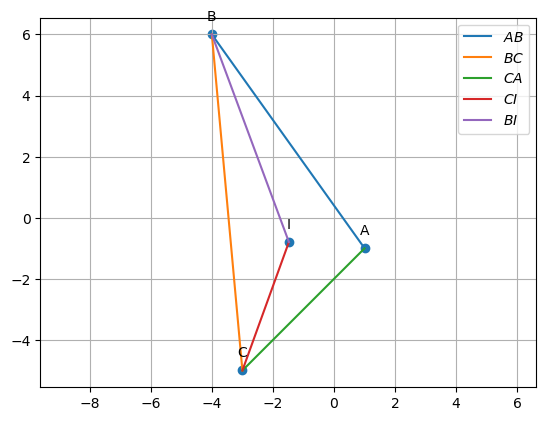
\includegraphics[width=\columnwidth]{./figs/Incentre.png}
\caption{Intersection point $\vec{I}$ of angle bisectors of $\vec{B}$and$\vec{C}$ plotted using python}
\label{fig:i_tri_py}
\end{figure}


